\section{Deep Neural Networks}
\begin{sectionbox}
\subsection{From Kernel to Neural Networks (NN)}
NN represent a methodology by which KERNELS are determined by means of a chosen learning method based on the available training data $\rightarrow$ KERNELS are composed by a concatenation of multiple VECTOR VALUED functions
\begin{emphbox}
$g(x)=f^{(L)}(f^{(L-1)}(...f^{(2)}(f^{(1)}(x;W^{(1)},v^{(1)});$\\
$W^{(2)},v^{(2)})...;W^{(L-1)},v^{(L-1)});W^{(L)},v^{(L)})$
\end{emphbox}
$f^{(l)}(*;W^{(l)},v^{(l)})\in \R^{N_t}$ represents the l-th layer of NN\\
NN consist of L+2 layers (INPUT Layer $x \in \R^N$ and LAYER OF OUTPUTS $f^{(NN)}\in \R^{N_{L+1}}$\\
HIDDEN LAYER (L=1) often enough\\
If $L>1$ NN is called \textbf{DEEP}\\

Mapping between NN layers consists typically of AFFINE TRANSFORMATION of the output of the preceding layer;\\
$\R^{N_{t-1}}\rightarrow \R{N_t}:f^{(l-1)} \rightarrow^{(l)}=W^{(l),T}f^{(l-1)}+v{(l)}$,\\
and the elementwise NONLINEAR TRANSFORMATION of the resulting INTERNAL STATE VECTOR $z^{(l)}$ by means of a NONLINEAR FUNCTION $\sigma^{(l)}$\\
\begin{emphbox}
$f^{(l)}(f^{(l-1)};W^{l}),v^{(l)})=\sigma^{(l)}(W^{(l),T}f^{(l-1)}+v^{(l)})$
\end{emphbox}

Elements of $^{(l)}$ and $v^{(l)}$ are called weights of the lth NN layer
\begin{itemize}
\item INPUT LAYER (l=0) of NN equals INPUT VECTOR $x \in \R^N$
\item OUTPUT LAYER (l=L+1) of NN equals OUTPUT VECTOR $f^{(NN)}\in \R^{N_{L+1}}$
\item NONLINEAR FUNCTION $\sigma_i^{(l)}$ of the HIDDEN LAYERS is different from the OUTPUT FUNCTION of the OUTPUT LAYER
\item latter depends on LOSS FUNCTION and the chosen LEARNING ALGORITHM
\end{itemize}

Single nonlinear function of the output vector of the previous layer composed by the i-th LINEAR FUNCTIONAL $w_i^{(l)}$, the CONSTANT $v_i^{(l)}$ and the i-th nonlinear function $\sigma^{(l)}$ of the next layer = NEURON. WEIGHTS represent the SYNAPTIC STRENGHTS and the nonlinear function $\sigma_i^{(l)}$ = ACTIVATION FUNCTION\\
\begin{emphbox}
$\sigma_i^{(l)}(\sum_{j=1}^{N_{(l-1)}}w_{i,j}^{(l)}f_j^{(l-1)}+v_i^{(l)})$

\end{emphbox}

\parbox{5.5cm}{\emph{Signal Neuron:} \\ 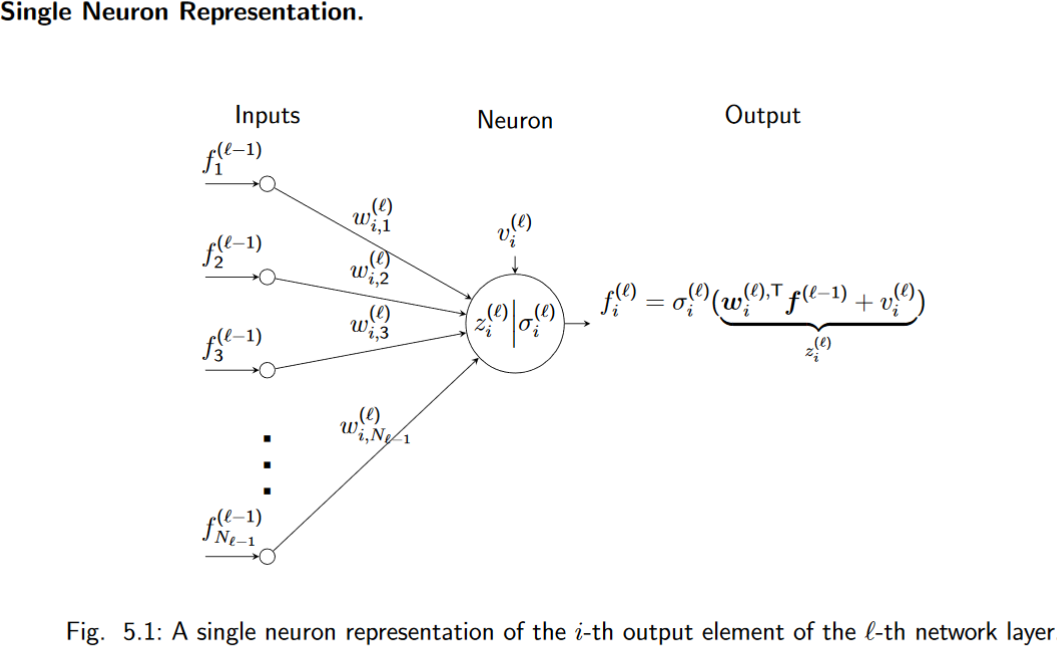
\includegraphics[width = 5.5cm]{./img/signalneuronrep}}

\parbox{5.5cm}{\emph{Neural Network:} \\ 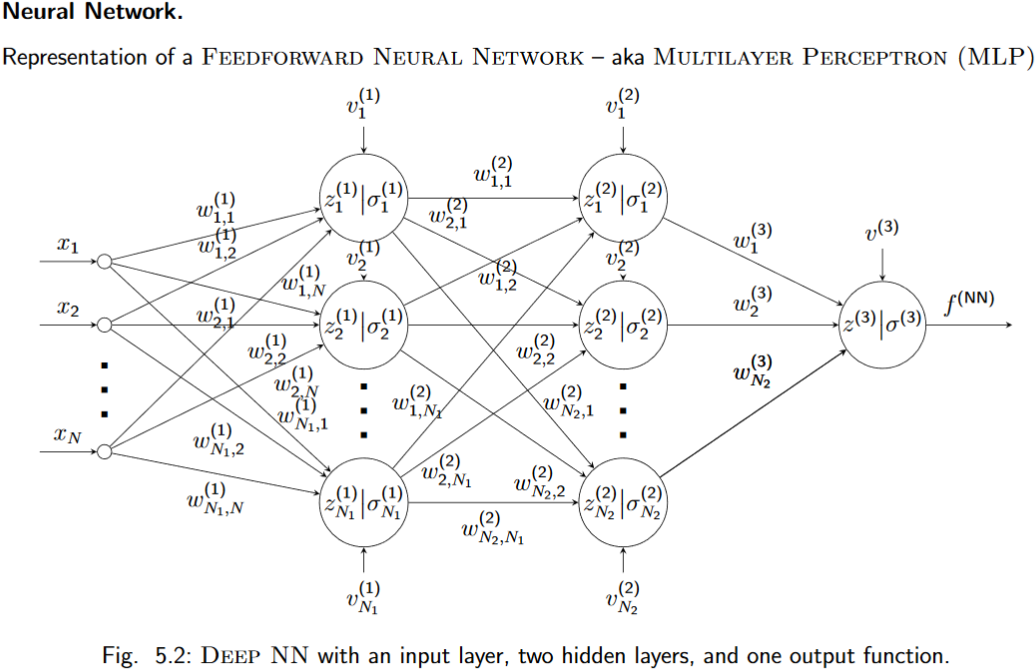
\includegraphics[width = 5.5cm]{./img/neuralnetwork}}
\end{sectionbox}
\begin{sectionbox}
\subsection{Activation Functions}
\subsubsection*{ReLU Activation Functions}
most popular chose for the activation function$\sigma_i^{(l)}\rightarrow$ RECTIFIED LINEAR UNIT FUNCTION (RELU)\\
\begin{emphbox}
$\sigma(z_i^{(l)})=max(0,z_i^{(l)})\in \R_+$\\
with $z_i{(l)}=sum_{j=1}^{N_{l-1}}w_{i,j}^{(l)}f_j^{(l-1)}+v_i^{(l)}$
\end{emphbox}
\begin{itemize}
\item PIECEWISE LINEAR FUNCTION which is zero for a negative state variable
\item efficient for the training of network weights, since its gradient with respect to the weight parameters does not experience any saturation for large positive values of the state variable, i.e.
\end{itemize}
\begin{emphbox}
$\frac{\partial \sigma(z_i^{(l)})}{\partial w_{i,j}^{(l)}}=\frac{\partial\sigma(z_i^{(l)})}{\partial z_i^{(l)}}\frac{\partial z_i^{(l)}}{\partial w_{i,j}^{(l)}}=unit(z_i^{(l)}f_j^{(l-1)})$ and\\
$\frac{\partial \sigma(z_i^{(l)})}{\partial v_{i,j}^{(l)}}=\frac{\partial\sigma(z_i^{(l)})}{\partial z_i^{(l)}}\frac{\partial z_i^{(l)}}{\partial v_{i,j}^{(l)}}=unit(z_i^{(l)})$\\
with the UNIT STEP FUNCTION unit(z)$\in{0,1}$
\end{emphbox}
\parbox{5.5cm}{\emph{RELU AF:}\\ 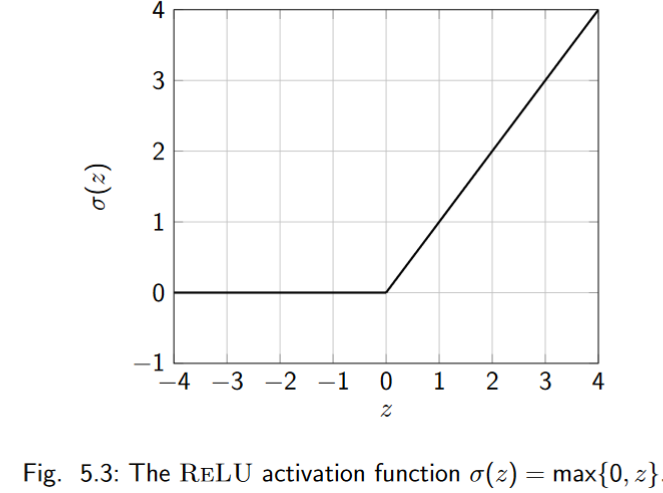
\includegraphics[width = 5.5cm]{./img/relu_af}}

\end{sectionbox}

\begin{sectionbox}
\subsubsection*{Hyperbolic Tangent Activation Functions}
Used to be standard before RELU
\begin{emphbox}
$ \sigma(z_i^{(l)})=tanh(z_i^{(l)})=\frac{e^{z_i^{(l)}}-e^{-z_i^{(l)}}}{e^{z_i^{(l)}}+e^{-z_i^{(l)}}} \in [-1,+1]$\\
with $z_i^{(l)}=\sum_{j=1}^{N_{l-1}}w_{i,j}^{(l)}f_j^{(l-1)}+v_i^{(l)}$
\end{emphbox}
The HYPERBOLIC TANGENT FUNCTION suffers from a saturation of its gradient with respect to weight parameters for large absolute values of the state variable, i.e.
\begin{emphbox}
$\frac{\partial \omega(z_i^{(l)})}{\partial w_{i,j}^{(l)}}=\frac{\partial\omega(z_i^{(l)})}{\partial z_i^{(l)}}\frac{\partial z_i^{(l)}}{\partial w_{i,j}^{(l)}}=(1-tanh^2(z_i^{(l)}))f_j^{(l-1)}$and\\
$\frac{\partial \omega(z_i^{(l)})}{\partial v_{i}^{(l)}}=(1-tanh^2(z_i^{(l)}))$
\end{emphbox}
Advantage: for small values of the state variable near $z_i^{(l)}=0$ the HYPERBOLIC TANGENT FUNCTION resembles a LINEAR MODEL\\

HYPERBOLIC TANGENT FUNCTION is very similiar to s.c. SIGMOID FUNCTION $\omega_{SIGMOID}(z_i^{(l)})=\frac{1}{1+e^{-z_i^{(l)}}}$\\
$\rightarrow tanh(z_i^{(l)})=2\sigma_{SIGMOID}(2z_i^{(l)})-1$\\

\parbox{5.5cm}{\emph{Hyperbolic Tangent AF:}\\ 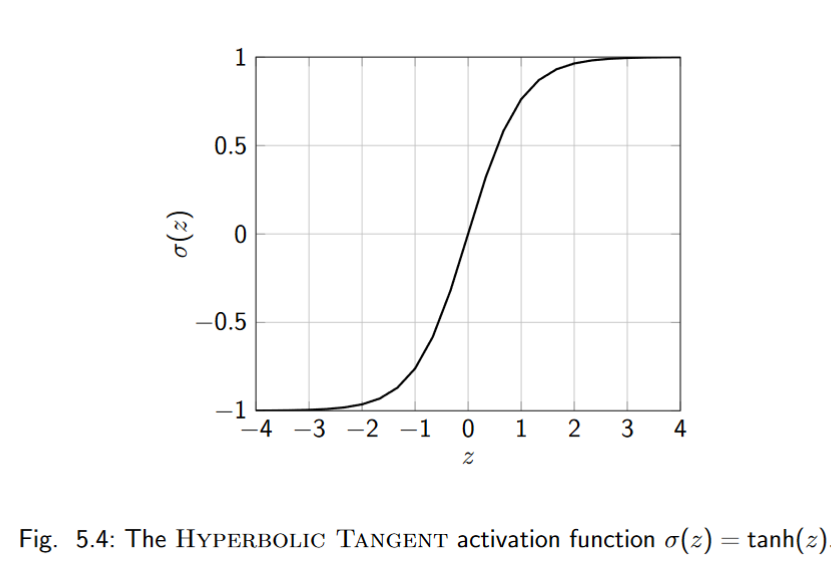
\includegraphics[width = 5.5cm]{./img/hyperbolic_tangent_af}}
\parbox{5.5cm}{\emph{Sigmoid AF:}\\ 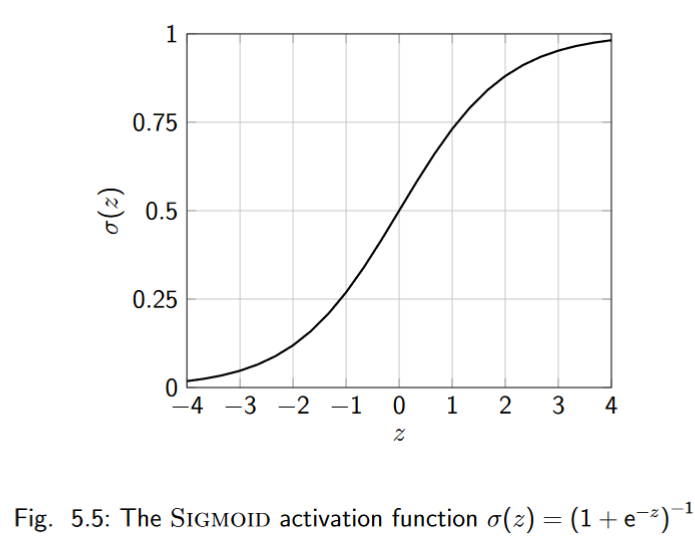
\includegraphics[width = 5.5cm]{./img/sigmoid_af}}
\end{sectionbox}
